\documentclass{article}

\usepackage{graphicx}
\usepackage{systeme}
\usepackage{mathabx}
\usepackage[T1]{fontenc}
\usepackage{listings}



\title{Lab 10}
\author{Filip Jędrzejewski}

\begin{document}
	\maketitle
	
	
	\section*{Opis problemu}

	Celem zadania było rozwiązanie bezczasowego równania Schrodingera:

	\begin{equation}
		\frac{1}{2} \left( \frac{\partial^2 \psi (x,y)}{\partial x^2} + \frac{\partial^2 \psi (x,y)}{\partial y^2} \right) + \frac{(n_1^2 + n_2^2) \pi ^2}{2L^2} \psi (x,y)
	\end{equation}

	przy czym:  \\
	$x \in (-\frac{L}{2}, \frac{L}{2})$ - pierwsza współrzędna położenia cząstki, \\
	$y \in (-\frac{L}{2}, \frac{L}{2})$ - druga współrzędna położenia cząstki, \\
	$\psi (x,y)$ - szukana funkcja falowa, \\
	$L$ - szerokość studni potencjału, \\
	$n_1$, $n_2$ - liczby kwantowe. \\

	Jednostki dobrano w ten sposób, że iloraz $\frac{h}{2\pi m} = 1$ oraz przyjęto, że $L = 2$. 

	\section*{Warunki brzegowe}

	Warunki brzegowe dla $|x| = \frac{L}{2}$ lub $|y| = \frac{L}{2}$:

	\begin{equation}
		\psi (x,y) = 0
	\end{equation}

	\section*{Rozwiązanie analitycze}

	Analityczna postać rozwiązania tego równania z powyższymi warunkami brzegowymi ma następującą postać:

	\begin{equation}
		\psi (x, y) = \frac{2}{L} \sin \left( \frac{n_1 \pi (x+\frac{L}{2})}{L} \right) \sin \left( \frac{n_2 \pi (y+\frac{L}{2})}{L} \right)
	\end{equation}


	\newpage

	\section*{Rozwiązanie korzystające z PINN}

	Zadanie rozwiązywano korzystając z biblioteki DeepXDE. 

	\subsection*{Importy i stałe}

	\begin{lstlisting}
import numpy as np
import deepxde as dde
import matplotlib.pyplot as plt

L = 2
	\end{lstlisting}

	\subsection*{Tworzenie dziedziny}

	\begin{lstlisting}
geometry1 = dde.geometry.Hypercube(xmin=[-L/2, -L/2, 0.99, 0.99], 
				   xmax=[L/2, L/2, 1.01, 1.01])
geometry2 = dde.geometry.Hypercube(xmin=[-L/2, -L/2, 1.99, 1.99], 
				   xmax=[L/2, L/2, 2.01, 2.01])

geometry = dde.geometry.CSGUnion(geometry1, geometry2)

geometry1 = dde.geometry.Hypercube(xmin=[-L/2, -L/2, 0.99, 1.99], 
				   xmax=[L/2, L/2, 1.01, 2.01])
geometry2 = dde.geometry.Hypercube(xmin=[-L/2, -L/2, 1.99, 0.99], 
				   xmax=[L/2, L/2, 2.01, 1.01])

geometry = dde.geometry.CSGUnion(geometry, geometry1)
geometry = dde.geometry.CSGUnion(geometry, geometry2)
	\end{lstlisting}

	\newpage

	\subsection*{Definicje funkcji}

	\begin{lstlisting}
def pde(x, u):
    du_xx = dde.grad.hessian(u, x, i=0, j=0)
    du_yy = dde.grad.hessian(u, x, i=1, j=1)
    n1 = x[:, 2:3]
    n2 = x[:, 3:4]
    return (du_xx + du_yy)/2 + (n1**2 + n2**2) * np.pi**2 * u / (2 * L**2)

def solution(x):
    xi = x[:, 0:1]
    yi = x[:, 1:2]
    n1 = x[:, 2:3]
    n2 = x[:, 3:4]
    
    return 2/L * np.sin(n1*np.pi*(xi+L/2) / L) * np.sin(n2*np.pi*(yi+L/2) / L)
	\end{lstlisting}

	\subsection*{Warunki brzegowe}

	\begin{lstlisting}
def boundaryFunction(x, on_boundary):
    if dde.utils.isclose(x[0], 0) or dde.utils.isclose(x[1], 0):
        return True
    if on_boundary and (dde.utils.isclose(abs(x[0]), L/2) 
			or dde.utils.isclose(abs(x[1]), L/2)):
        return True
    return False



boundary_conditions = dde.icbc.DirichletBC(geometry, 
                                            lambda x: solution(x), 
                                            boundaryFunction
                                            )
	\end{lstlisting}

	\subsection*{Tworzenie danych}

	\begin{lstlisting}
data = dde.data.PDE(geometry, 
                    pde, 
                    boundary_conditions, 
                    num_domain=3000,
                    num_boundary=5000,
                    num_test=1500
                    )
	\end{lstlisting}

	\subsection*{Definiowanie sieci}

	\begin{lstlisting}
net = dde.nn.FNN([4]+[30]*2+[1],
                "tanh",
                "Glorot normal"
                )

	\end{lstlisting}


	\subsection*{Tworzenie modelu}

	\begin{lstlisting}
model = dde.Model(data, net)

model.compile("adam", lr=0.01)
	\end{lstlisting}

	\subsection*{Trenowanie modelu}

	\begin{lstlisting}
loss_history, train_state = model.train(iterations = 1500, display_every=500)
dde.saveplot(loss_history, train_state, issave=False, isplot=True)
	\end{lstlisting}
	
	\newpage

	\subsection*{Wykres funkcji kosztu w zależności od liczby iteracji}

	\begin{figure}[h]
		\centering
		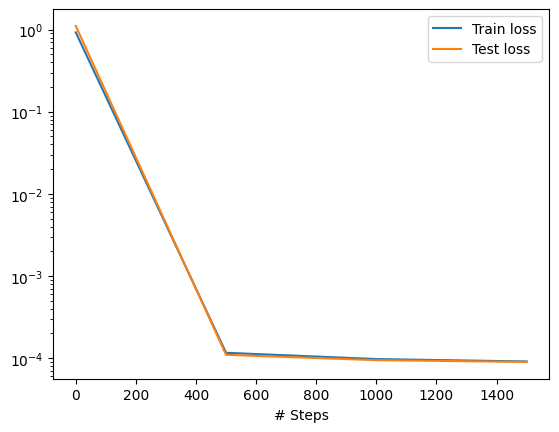
\includegraphics[scale = 0.70]{wykres1.png}
	\end{figure}
	

	\section*{Wykresy}

	\subsection*{Kod}

	\begin{lstlisting}
xData = np.linspace(-L/2, L/2, 1000)
yData = np.linspace(-L/2, L/2, 1000)
n1 = np.array([1 for i in range(1000)])
n2 = np.array([1 for i in range(1000)])
		
X = np.vstack((np.ravel(xData), np.ravel(yData), np.ravel(n1), np.ravel(n2))).T
		
		
y_pred = model.predict(X)
		
y_true = solution(X)

plt.plot(X[:, 0:1], y_pred)
plt.plot(X[:, 0:1], y_true)
plt.show()
	\end{lstlisting}

	\subsection*{Wykresy funkcji $\psi (x, y)$ oraz jej przybliżenia znalezionego przez sieć}

	\begin{figure}[h]
		\centering
		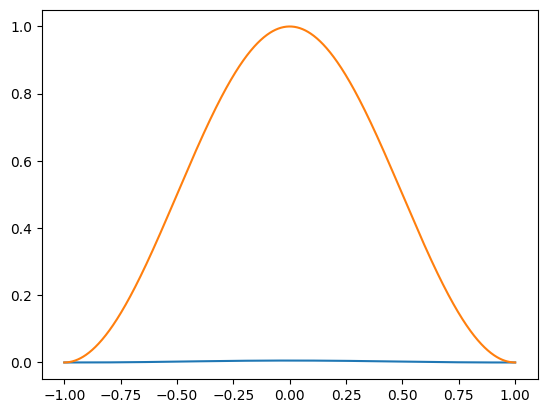
\includegraphics[scale = 0.70]{wykres2.png}
	\end{figure}

	linia pomarańczowa - rozwiązanie analityczne, 
	linia niebieska - rozwiązanie znalezione przez sieć.

	\newpage

	\subsection*{Wykres błędu względnego}

	\begin{lstlisting}
errors = abs(y_pred - y_true) / y_true
plt.plot(X[:, 0:1], errors)
plt.show()
	\end{lstlisting}

	\begin{figure}[h]
		\centering
		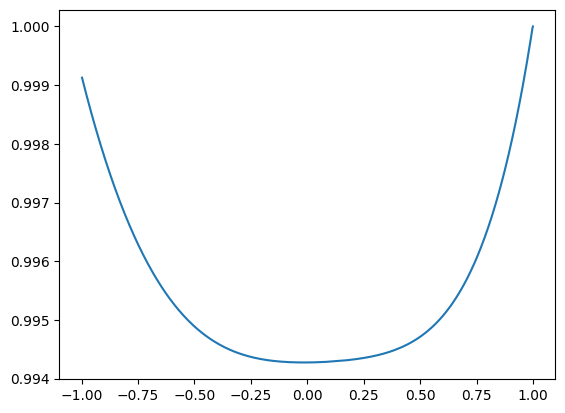
\includegraphics[scale = 0.70]{wykres3.png}
	\end{figure}


	

	
	
	
\end{document}